\documentclass[b5paper,twoside]{article}

\usepackage[T1]{fontenc}
\usepackage{kpfonts}

\usepackage{amsmath,amsthm,amsfonts,amssymb}
\usepackage{mathrsfs}
\usepackage[scr=boondoxo]{mathalfa}
\usepackage{thmtools, thm-restate}
\usepackage{titling}
\usepackage{tikz}
\usepackage{tikz-cd}
\usepackage{tikzsymbols} 
\usetikzlibrary{arrows.meta,decorations.pathmorphing,backgrounds,positioning,fit,petri}
\usepackage{comment}
\usepackage[newparttoc]{titlesec}
\usepackage{titletoc}
\usepackage{indentfirst}
\usepackage{graphicx}
\usepackage{float}
\usepackage{tabulary}
\usepackage{ifthen}
\usepackage[nottoc]{tocbibind}
%\usepackage{hyperref}
\usepackage[colorlinks=true]{hyperref}
\hypersetup{linkcolor=red,urlcolor=red,citecolor=green}
\usepackage{cleveref}
\usepackage{stmaryrd}
%\usepackage{xcolor}
%\usepackage{cancel}
%\usepackage{anyfontsize}
%\usepackage{imakeidx}
%\usepackage{soul}
%\usepackage{ulem}
%\setlength\parindent{0pt}

\makeatletter
\let\newtitle\@title
\let\newauthor\@author
\let\newdate\@date
\makeatother

\usepackage{geometry}
\geometry{
	top=0.75in, 
	bottom=0.75in, 
	left=0.75in, 
	right=0.75in, 
	includehead, 	
}

\usepackage{fancyhdr}
\pagestyle{fancy}
\renewcommand\sectionmark[1]{\markboth{\S\,\thesection\enskip#1}{}}

%\renewcommand{\headrulewidth}{0pt}
\fancyhead{}
\fancyhead[LE,RO]{\oldstylenums{\thepage}}
\makeatletter
\fancyhead[RE]{\newtitle}
\fancyhead[LO]{\newtitle}
\makeatother
\fancyfoot{}
\setlength{\parindent}{0pt}

\titleformat{\section}[block]{\Large\bfseries\scshape}{\S\,\thesection}{.5em}{\filcenter}
\titleformat{\subsection}[block]{\normalsize\bfseries\scshape}{\S\,\thesubsection}{.5em}{\filright}

\renewcommand\thesection{\oldstylenums{\arabic{section}}}
\renewcommand\thesubsection{\oldstylenums{\arabic{section}.\arabic{subsection}}}

\renewcommand\contentsname{Table of Contents}

\titlecontents{section}[0pt]{\normalsize\scshape}{\S\,\thecontentslabel\enskip}{}{\titlerule*[8pt]{.}\oldstylenums{\contentspage}}
\titlecontents{subsection}[12pt]{\small\scshape}{\S\,\thecontentslabel\enskip}{}{\titlerule*[8pt]{.}\contentspage}


\newtheoremstyle{akari}{}{}{\itshape}{}{\upshape\bfseries\scshape}{.\;}{ }{\thmnote{#3}}
\newtheoremstyle{yui}{}{}{}{}{\upshape\bfseries}{.\;}{ }{\thmnumber{(#2) }{\scshape\thmname{#1}}\thmnote{ (#3)}}
\newtheoremstyle{kyoko}{}{}{\itshape}{}{\upshape\bfseries}{.\;}{ }{\thmnumber{(#2) }{\scshape\thmname{#1}}\thmnote{ (#3)}}
\newtheoremstyle{kyoko*}{}{}{\itshape}{}{\upshape\bfseries}{.\;}{ }{{\scshape\thmname{#1}}\thmnote{ (#3)}}
\newtheoremstyle{chinatsu}{}{}{}{}{\upshape\bfseries}{.\;}{ }{{\scshape\thmname{#1}}\thmnumber{ #2}\thmnote{ (#3)}}

\theoremstyle{kyoko}
\newtheorem{theorem}{Theorem}[section]
\newtheorem{apptheorem}{Theorem}[section]
\renewcommand\thetheorem{\oldstylenums{\arabic{section}.\arabic{theorem}}}
\renewcommand\theapptheorem{\Alph{section}.\oldstylenums{\arabic{apptheorem}}}
\newtheorem{proposition}[theorem]{Proposition}
\newtheorem{appproposition}[apptheorem]{Proposition}
\newtheorem{corollary}[theorem]{Corollary}
\newtheorem{appcorollary}[apptheorem]{Corollary}
\newtheorem{lemma}[theorem]{Lemma}
\newtheorem{applemma}[apptheorem]{Lemma}
\newtheorem{conjecture}[theorem]{Conjecture}
\newtheorem{appconjecture}[apptheorem]{Conjecture}

\theoremstyle{kyoko*}
\newtheorem*{theorem*}{Theorem}
\newtheorem*{proposition*}{Proposition}
\newtheorem*{lemma*}{Lemma}

\theoremstyle{yui}
\newtheorem{definition}[theorem]{Definition}
\newtheorem{appdefinition}[apptheorem]{Definition}
\newtheorem{notation}[theorem]{Notation}
\newtheorem{example}[theorem]{Example}
\newtheorem{appexample}[apptheorem]{Example}
\newtheorem{situation}[theorem]{Situation}
\newtheorem{remark}[theorem]{Remark}
\newtheorem{appremark}[apptheorem]{Remark}

\theoremstyle{chinatsu}
\newtheorem{exercise}{Exercise}
\renewcommand\theexercise{\oldstylenums{\arabic{exercise}}}

\theoremstyle{akari}
\newtheorem*{akari}{}

\renewcommand{\theenumi}{\oldstylenums{\arabic{enumi}}}
\renewcommand{\labelenumi}{(\theenumi)}

\renewcommand{\theenumii}{\alph{enumii}}
\renewcommand{\labelenumii}{(\theenumii)}

\renewcommand{\theenumiii}{\roman{enumiii}}
\renewcommand{\labelenumiii}{(\theenumiii)}

\renewcommand*{\proofname}{\upshape\scshape\bfseries Proof}
\renewcommand{\qedsymbol}{$\blacksquare$}

%\renewcommand\bibname{BIBLIOGRAPHY}

\tikzcdset{
    row sep/normal=3.6em,
    column sep/normal=3.6em,
    arrows=semithick,
    arrow style=tikz,
    diagrams={>={Stealth[round]}}
}

\tikzset{
    pre/.style={<-,shorten <=1pt,>={Stealth[round]},semithick},
    post/.style={->,shorten >=1pt,>={Stealth[round]},semithick}
}



\tikzcdset{
    row sep/normal=3.6em,
    column sep/normal=3.6em,
    arrows=semithick,
    arrow style=tikz,
    diagrams={>={Stealth[round]}}
}

\tikzset{
    pre/.style={<-,shorten <=1pt,>={Stealth[round]},semithick},
    post/.style={->,shorten >=1pt,>={Stealth[round]},semithick}
}

\title{\scshape Assignment \oldstylenums{1} - MVP's}
\author{
    \scshape Lindi Li \\ \oldstylenums{3460570} \and
    \scshape Gewei Cao \\ \oldstylenums{3461232}
}
\date{December \oldstylenums{2022}}


\begin{document}

\maketitle

\section{Intrudction}
blabla

\section{Reproducing Kernel Hilbert Space} 

\subsection{Hilbert Space}
Recall that an inner product $<a,b>$ can be
\begin{itemize}
    \item a usual dot product: $<a,b>=a'b=\sum_i a_i b_i$.
    \item a kernel product: $<a,b>=k(a,b)=\psi(a)'\psi(b)$, where $\psi(a)$ may have infinite dimensions.
\end{itemize} 
A normed space is a vector space $N$ on which a norm is defined. A nonnegative function $\parallel\cdot\parallel$ is a norm if and only if $\forall f,g\in N$ and $\alpha\in\mathbb{R}$:
\begin{itemize}
    \item $\parallel f \parallel \geq 0$ and $\parallel f\parallel=0$ iff $f=0$;
    \item $\parallel f+g \parallel \leq \parallel f \parallel + \parallel g \parallel$;
    \item $\parallel \alpha f\parallel=\mid \alpha \mid & \parallel f \parallel$
\end{itemize}
Now we can define a Hilbert space an inner product space that is complete and separable with respect to the norm defined by inner product.
An example of a defined norm in Hilbert space (i.e, the space $L_2$ of square integrable functions) can be 
\begin{equation}
    \parallel f \parallel = \left(\int_a^b f^2(t)dx\right)^\frac{1}{2}.
\end{equation}

\subsection{Kernel Method}
The motivation of kernel method is simple. Imagine there are some blue dots and red dots on a vector space $\mathbb{R}^n$ and 
we want to separate them by color. As it shows in the left hand side figure, it is difficult to divide them through a straight 
line. However, we may be able to separate them easily by mapping each dot into a high-dimension feature space. The figure below 
shows how mapping works:
\begin{figure}[H]
    \centering
    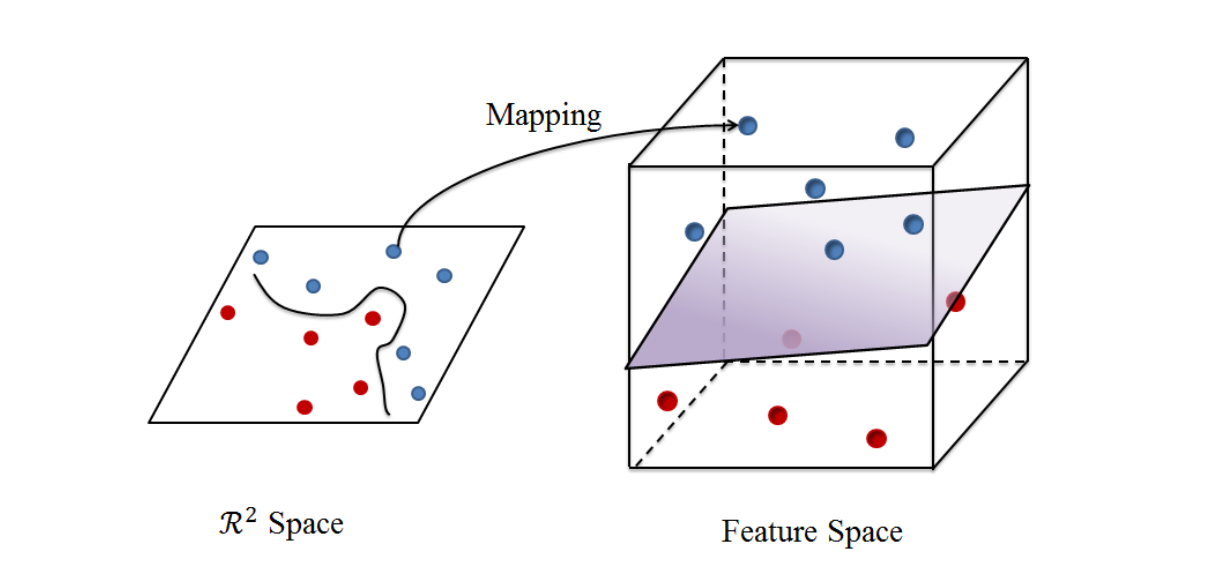
\includegraphics[width=0.7\textwidth]{Mapping}
\end{figure}
Let's now use a simple example to illustrate the idea of kernel method. 
we set two vectors $\textbf{x}=\begin{bmatrix}x_1&x_2\end{bmatrix}$ and $\textbf{y}=\begin{bmatrix}y_1&y_2\end{bmatrix}$ in a two-dimension space.
Tow functions $\phi(x)$ and $\phi(y)$ are defined as:
\begin{equation*}
    \phi(x)=\begin{bmatrix}
        x_1x_1&x_1x_2&x_2x_1&x_2x_2
    \end{bmatrix}
\end{equation*}
\begin{equation*}
    \phi(y)=\begin{bmatrix}
        y_1y_1&y_1y_2&y_2y_1&y_2y_2
    \end{bmatrix}
\end{equation*}
We now successfully mapping them into a four-dimension feature space. Therefore, instead of computing the inner product of $<\phi(x),\phi(y)>$, we can define 
a corresponding kernel function $K(\textbf{x},\textbf{y})=<\textbf{x},\textbf{y}>^2$. It can be easily proofed that $K(\textbf{x},\textbf{y})$ is the same as $<\phi(\textbf{x}),\phi(\textbf{y})>$:
\begin{align*}
    K(\textbf{x},\textbf{y})&=<\textbf{x},\textbf{y}>^2\\
                            &=(x_1y_1+x_2y_2)^2\\
                            &=x_1^2y_1^2+2x_1y_2x_2y_1+x_2^2y_2^2\\
                            &=<\phi(\textbf{x}),\phi(\textbf{y})>
\end{align*}
To write the above example in a general form, we first set an equation where $\phi(\cdot)\in\mathbb{R}^m$ and $\phi(x)$ is defined as the mapping function:
\begin{align}
    y&=\phi(x)^\top w \notag\\
     &= \begin{bmatrix}
        \phi_1(x) \\
        \vdots \\
        \phi_m(x)
        \end{bmatrix} w \notag\\
     &= \begin{bmatrix}
        \phi_1(x)\cdots\phi_m(x)
        \end{bmatrix} w
\end{align}
$Y$ and $\Phi$ in generalization is defined by:
\begin{equation}
    Y=\begin{bmatrix}
         y_1&\cdots&y_n
      \end{bmatrix}^\top 
\end{equation}
\begin{align}
    \Phi&=\begin{bmatrix}
           \phi(x_1)&\cdots&\phi(x_n) 
          \end{bmatrix}^\top \notag\\
        &=\begin{bmatrix}
           \phi_1(x_1)&\cdots&\phi_m(x_1)\\
           \vdots&\vdots&\vdots \\
           \phi_1(x_n)&\cdots&\phi_m(x_n)
          \end{bmatrix}
\end{align}
In most of the cases, we want to avoid computing $\phi(x)$ in a explicit way, especially when $m$ is very large. Therefore, we define a kernel function:
\begin{equation}
    [\Phi\Phi^(top)]_{i,j}=\phi(x_i)^(top) \phi(x_j)=K(x_i,x_j)
\end{equation}
$\phi(x_i)^top\phi(x_j)$ is usually very difficult to compute, and thus we use $\mathbb{K}(x_i,x_j)$ to replace.

In the simplest form of machine learning, in order to predict $x$, the algorithm collects the samples in the training set $\chi$ that are similar to $x$, 
and then take the weighted value of these samples as the predict value of $x$. Here comes the questions:
\begin{itemize}
    \item How to measure the similarity between samples?
    \item How to weight the value of each sample?
\end{itemize} 
In general, the higher the similarity of the sample to our point of interest $x$, the more the sampling weights. To evaluate the similarity between two observations, 
a kernel is defined as a function of two input patterns $k(x_i, x_j)$, mapping onto a real-valued output. For example, the Gaussian kernel is
\begin{equation}
    k(x_i, x_j) = e^\frac{\parallel x_i - x_j \parallel}{\sigma^2},
\end{equation}
where $\parallel x_i - x_j \parallel$ is the Euclidean distance between $x_i$ and $x_j$, and $\sigma^2 \in \mathbb{R}^+$ is the bandwidth of the kernel function.\\
We now define that $k: \chi \times \chi \rightarrow \mathbb{R}$ is a kernel if
\begin{itemize}
    \item $k$ is symmetric: $k(x,y) = k(y,x)$.
    \item $k$ is positive semi-definite, meaning that $\sum_{i} \sum_{j} \alpha_i \alpha_j k(x_i,x_j)\geq0, \forall \alpha_i, \alpha_j \in \mathbb{R}, x \in \mathbb{R}^\mathbb{D}, D \in \mathbb{Z}^+$. 
    \item We define the corresponding kernel matrix as the matrix $K$ with entries $k_{ij}=k(x_i,x_j)$, the sencond property of $k$ is equivalent to saying that $c'Kc \geq0$.
\end{itemize}
From the similarity-based point of view, the use of kernels for regression can be described in two stages. We set $y_i \in \mathbb{R}$ as dependent variable, 
and $x_i$ as a $1 \times D$ vector $x_i \in \mathbb{R}^D$ of covariate values. Assume that $(y_i, x_i)$ where $i = 1, \dots, N$ is i.i.d. We first define a target function $y=f(x)$ and assume that in a space of functions, there exists 
a function that can estimate $y=f(x)$ well. The target function could be represented by
\begin{equation}
    f(x)= \sum_{i=1}^N w_i k(x,x_i),
\end{equation}
A perfect solution to estimate N parameters for N observations would be choosing $\hat{w}=K^{-1}y$. However, such a fit could result in extremely high variance. Therefore, we impose an addtional assumption 
that a smoother curve with less oscillations is prefered. We then utilize regularization to simplify the function and satisfy the additional assumption in 
the second stage. To achieve this purpose, Hilbert space and reproducing kernel Hilbert space will be introduced below.





\section{Bayies}
blabla

\section{Empirical study}
blabla

\end{document}